\chapter{TVN/GTE: Local Field Potentials}
\label{chap:LFP}
\ghnote{Torbjorn will take the main responsibility for this chapter}
\tvnnote{Add brief historical perspective, Gaute? Bliss and L\o mo, 1973 used it to discover LTP, many have studies oscillations, might be good for BMI etc.}

%\subsection{\red{Introduction to Local Field Potentials}}
Extracellular potentials measured in neural tissue reflects extracellular spikes, vast numbers of synaptic inputs, as well as different types of noise. The Local Field Potential (LFP) is the low-frequency part of these extracellular potentials, found by low-pass filtering the recorded signals below $\lesssim$ 500~Hz. The LFP is thought to primarily reflect synaptic inputs to populations of geometrically aligned pyramidal cells.

\begin{figure}[!ht]
\begin{center}
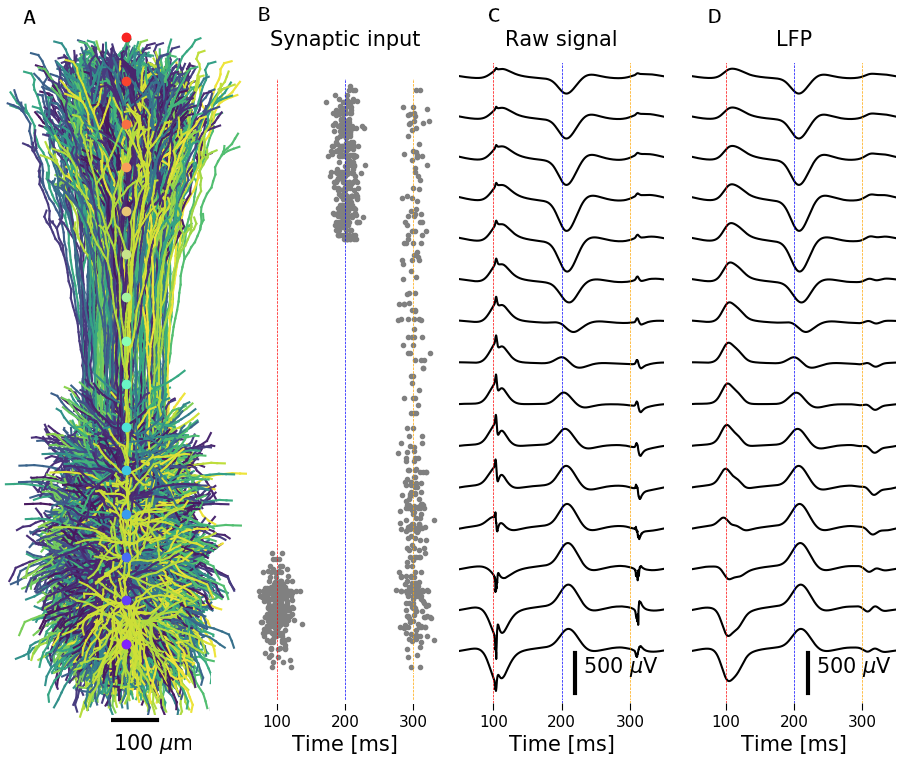
\includegraphics[width=.7\textwidth]{Figures/LFP/population_LFP.png}
\end{center}
\caption{\textbf{Illustration the origin of the LFP.}
Synaptic input to a population of 10 000 pyramidal cells.
}
\label{fig:LFP:LFP_pop_origin}
\end{figure}




\section{\red{The dipolar nature of LFP signals}}
The LFP is thought to reflect synaptic inputs to thousands of pyramidal neurons, and the contribution to the LFP from any single neuron is typically considered negligible. However, a lot of qualitatively important insights about the biophysical origin of the LFP can still be gained from considering synaptic input to single neurons. 

\begin{figure}[!ht]
\begin{center}
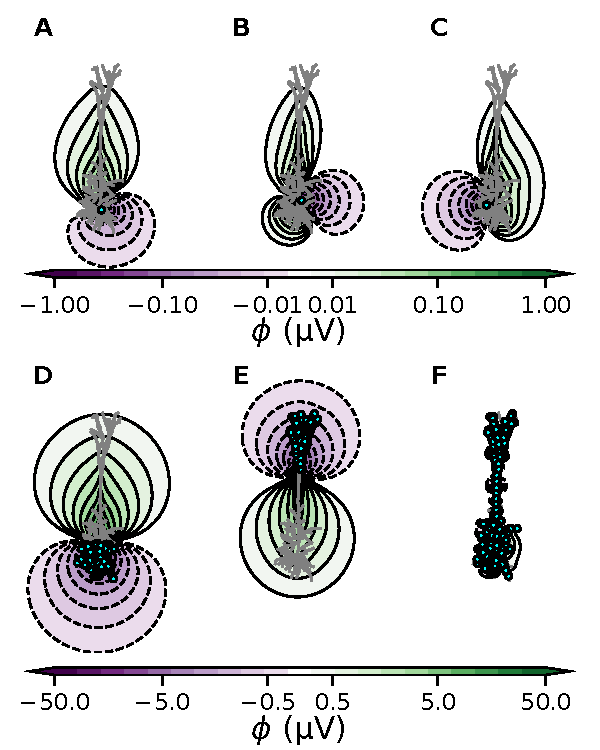
\includegraphics[width=.6\textwidth]{Figures/LFP/fig_chosen_dipoles.pdf}
\end{center}
\caption{\textbf{LFPs from synaptic inputs to pyramidal cell}
Snapshot of the LFP around a neuron model from synaptic input (cyan dots). LFPs stemming from different synaptic input locations can be highly variable ({\bf A-C}), but many synaptic inputs to specific cell regions give more standardized LFP responses ({\bf D-E}). Uniformly distributed synaptic inputs will tent to lead to more or less random source/sink distributions, and much weaker LFPs.
}
\label{fig:LFP:LFP_dipoles}
\end{figure}


One of the defining features of the LFP is its dipolar nature. This stems from current conservation, implying that current going into the cell at one location is exactly balanced by current going out of the cell at other locations, so that synaptic input always gives rise to a balanced set of current sources and sinks (see \fref{chap:Neuron}). The simulated LFP in the vicinity of a neuron stemming from a single synaptic input can be highly irregular in shape due to the morphological details of the cell. For example, different locations of a single excitatory synaptic inputs to the basal dendrite of a pyramidal cell can not be expected to result in similar LFPs, and will not necessarily be dipolar in shape (\fref{fig:LFP:LFP_dipoles}{\bf A-C}). However, for many simultaneous excitatory synaptic inputs to the basal dendrite of a pyramidal cell, we can expect that the irregularities largely cancel, and that the resulting LFP will be dominated by a basal sink (excitatory input gives negative transmembrane currents), and an apical source (\fref{fig:LFP:LFP_dipoles}{\bf D}). Similarly, many excitatory synaptic inputs to the apical dendrite of a pyramidal cell can be expected to result in an apical sink and a basal source (\fref{fig:LFP:LFP_dipoles}{\bf E}). Finally, synaptic input that is uniformly spread out over an entire neuronal morphology will tend to cause a more or less random distribution of current sources and sinks, leading to strong cancellations in the LFP and not in a dipolar shape of the LFP (\fref{fig:LFP:LFP_dipoles}{\bf F}) (but see also sec. XX (Ih)). 



\section{\red{Strong LFP signals require asymmetry}}
From the analysis in the previous paragraph, we can draw important conclusions about the origin of the LFP. 			
Firstly, synaptic inputs to a population of neurons will cause much stronger LFP signals if the synaptic input is asymetrically distributed on the neurons. 
This can happen if a given pre-synaptic neural population has a preferential synaptic target region on a given post-synaptic population. It is for example known that the inhibitory cortical Martinotti cells tend to make synaptic contacts on the distal apical dendrites of pyramidal neurons. 
Note that this can only happen if the post-synaptic population has a certain geometrical alignment of its neurons with distinct cell regions, like basal and apical dendrites. In cortex, the inhibitory interneurons and excitatory layer 4 stellate cells tend to be more symmetrical than pyramidal cells, and their morphologies are not as clearly separated into different cell regions. This prevents the asymmetric distribution of synapses that is needed for generating strong LFP signals \cite**{Linden2011,Hagen2016,Naess2020}.
\tvnnote{Make illustration figure, similar to but simpler than Fig 4 in N\ae ss et al 2021?}
\tvnnote{Er dette for bastant? Tar kanskje ikke hoyde for situasjonen fra Swadlow2002/Hagen2017?}

Since there is reason to believe that the LFP is dominated by asymmetric synaptic input to geometrically aligned populations of pyramidal cells, we can identify four main LFP contributors: excitatory or inhibitory synaptic input to the apical or basal dendrites, see \fref{fig:LFP:LFP_lego}.

\begin{figure}[!ht]
\begin{center}
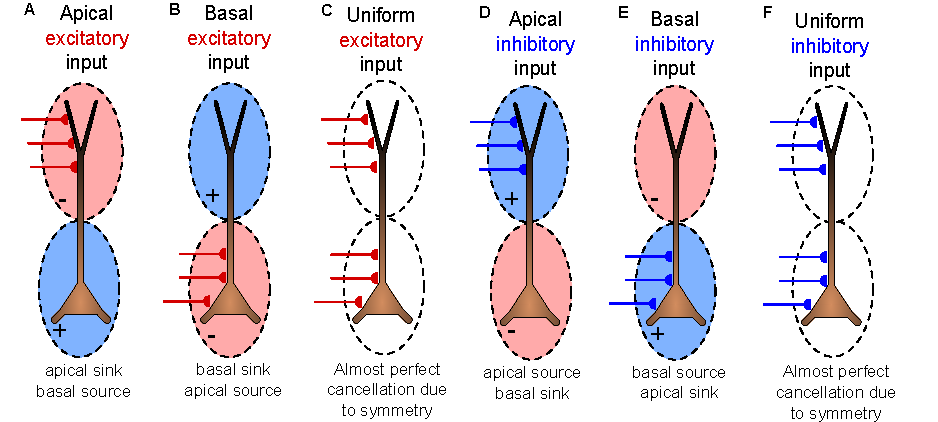
\includegraphics[width=.7\textwidth]{Figures/LFP/dipole_basics.pdf}
\end{center}
\caption{\textbf{Basic building blocks of the LFP.}
Illustration of the LFP at a snapshot in time in a region around a pyramidal
cell in response to different types of synaptic input. The LFP signature depends on the type of synaptic input (excitatory or inhibitory), and the location (apical, basal, uniform), but also, to a lesser degree, to many other parameters of the cells and synapses.
}
\label{fig:LFP:LFP_lego}
\end{figure}

\section{\red{Morphology matters}}
\label{sec:LFP:morph_matters}

The LFP generated by synaptic input to a neuron is very dependent on the morphology, since the morphology fundamentally shapes the distribution of return currents. 
Pyramidal neurons typically has a basal dendritic structure with neurites extending out from the soma in all directions, but the most characteristic feature of pyramidal cells is the apical dendrite, which is thicker and can often be up to a couple of millimeters long.
For a simulated example of the LFP in the vicinity of a experimentally reconstructed pyramidal cell receiving a single synaptic input to the soma, see \fref{fig:LFP:morph_matters}{\bf A}. We see that there is a strong negative deflection concentrated around the somatic region, and a weaker and more distributed positive deflection upwards along the apical dendrite. If we look at the normalized shape of the LFP signal with increasing distance from the soma, we see that the LFP response gets broader with distance (\fref{fig:LFP:morph_matters}{\bf A}; bottom) (more on this later).

The apical dendrite is important for the LFP, but for some purposes, the other dendrites can be neglected, resulting in a simplified ball and stick model. As seen in \fref{fig:LFP:morph_matters}{\bf B}, this model can reproduce many of the features described for the experimentally reconstructed neuron model.

Simplifying this further leads us to a two compartment model  (\fref{fig:LFP:morph_matters}{\bf C}),
which is the simplest possible model which can generate extracellular potentials.  
Far away from the neuron, this two-compartment model can give accurate results for LFP signals (see EEG chapter, \fref{chap:EEG}), but it fails to reproduce many features of the LFP,
like the increased with of the LFP from synaptic input with increasing distance.


\begin{figure}[!ht]
\begin{center}
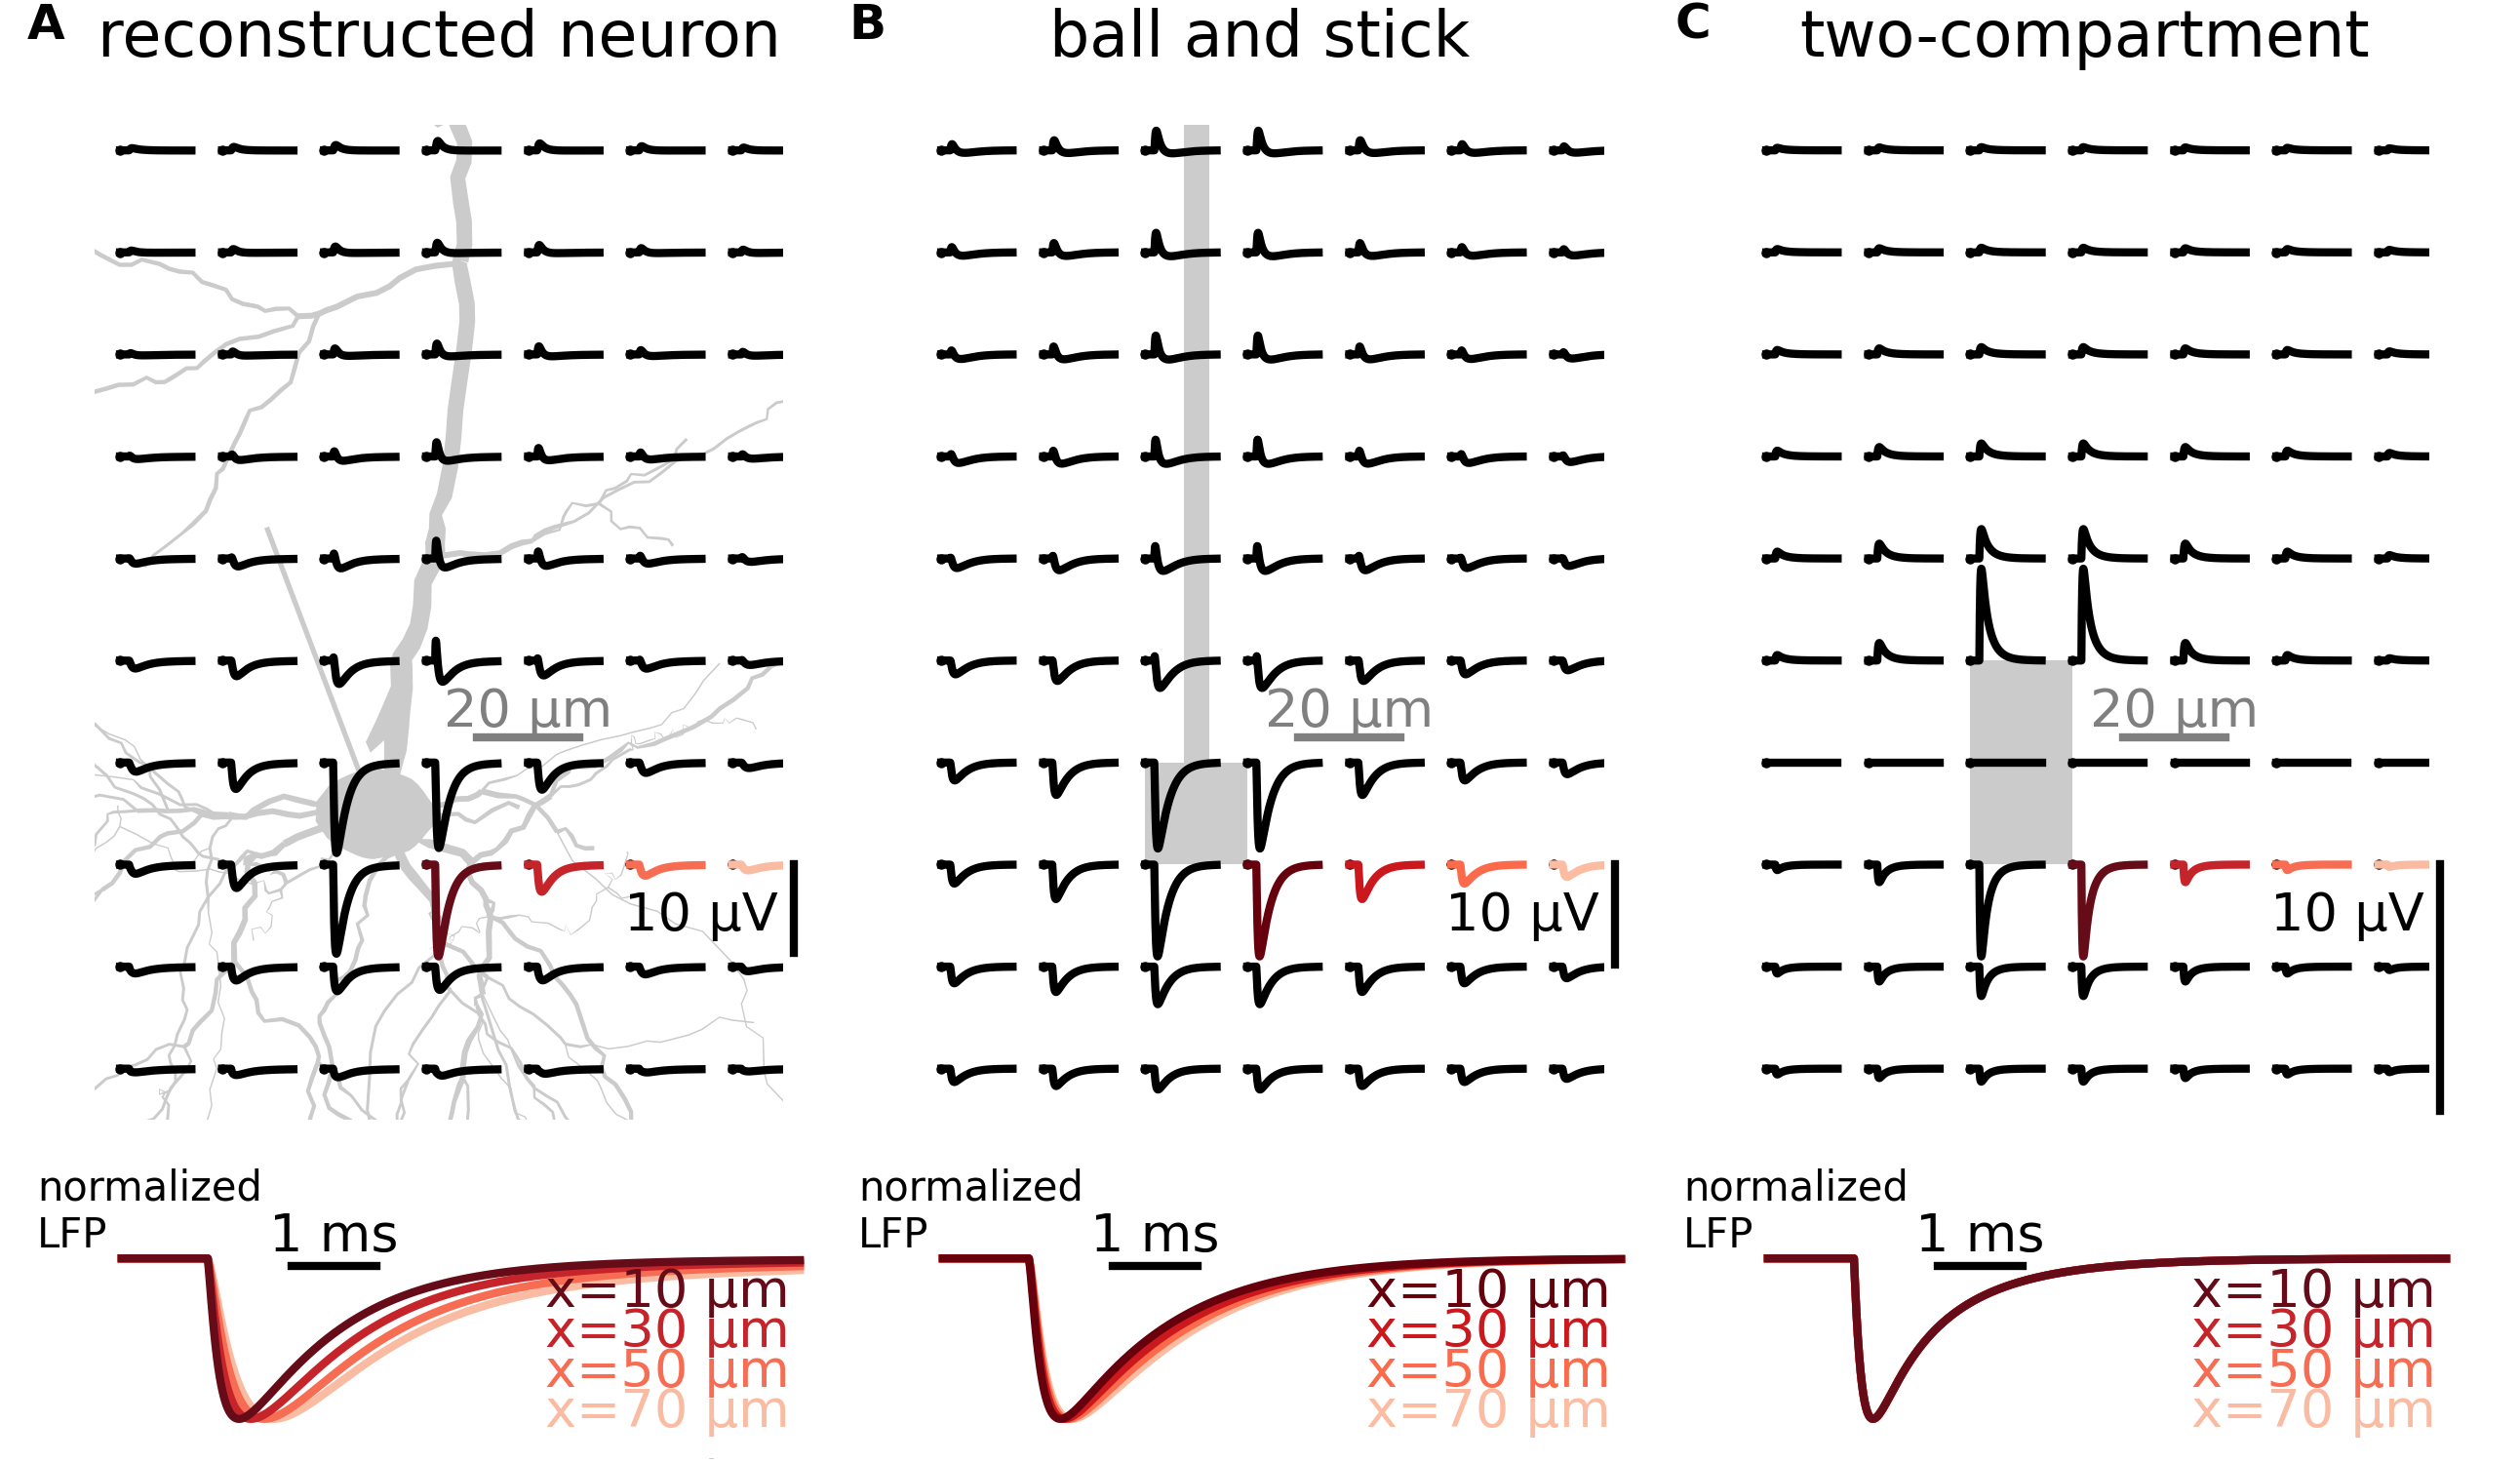
\includegraphics[width=1.\textwidth]{Figures/LFP/compare_hay_bns_2comp.png}
\end{center}
\caption{\textbf{The shape of the LFP signal is dependent on the morphology.}
Synaptic input to the 'soma' for three different types of model morphology. The LFP is always kind of dipolar, but there's more to it. Signal becomes wider for reconstructed morphology, but not for two-compartment model.
%\cite**{Hay2011}
}
\label{fig:LFP:morph_matters}
\end{figure}





\section{\red{Frequency-content of LFP signals}}
\label{sec:LFP:freq_content}

LFPs are often analyzed in terms of the frequency content.
A clean way of illustrating the effect of the cellular morphology on the frequency-content of LFP signals
is through injecting a white noise current. A white noise current by definition has equal amplitude at all frequencies, and its power spectral density (PSD) spectrum is therefore flat.
Again, we can see that Morphology still matters (\fref{fig:LFP:morph_matters_PSD}).

\begin{figure}[!ht]
\begin{center}
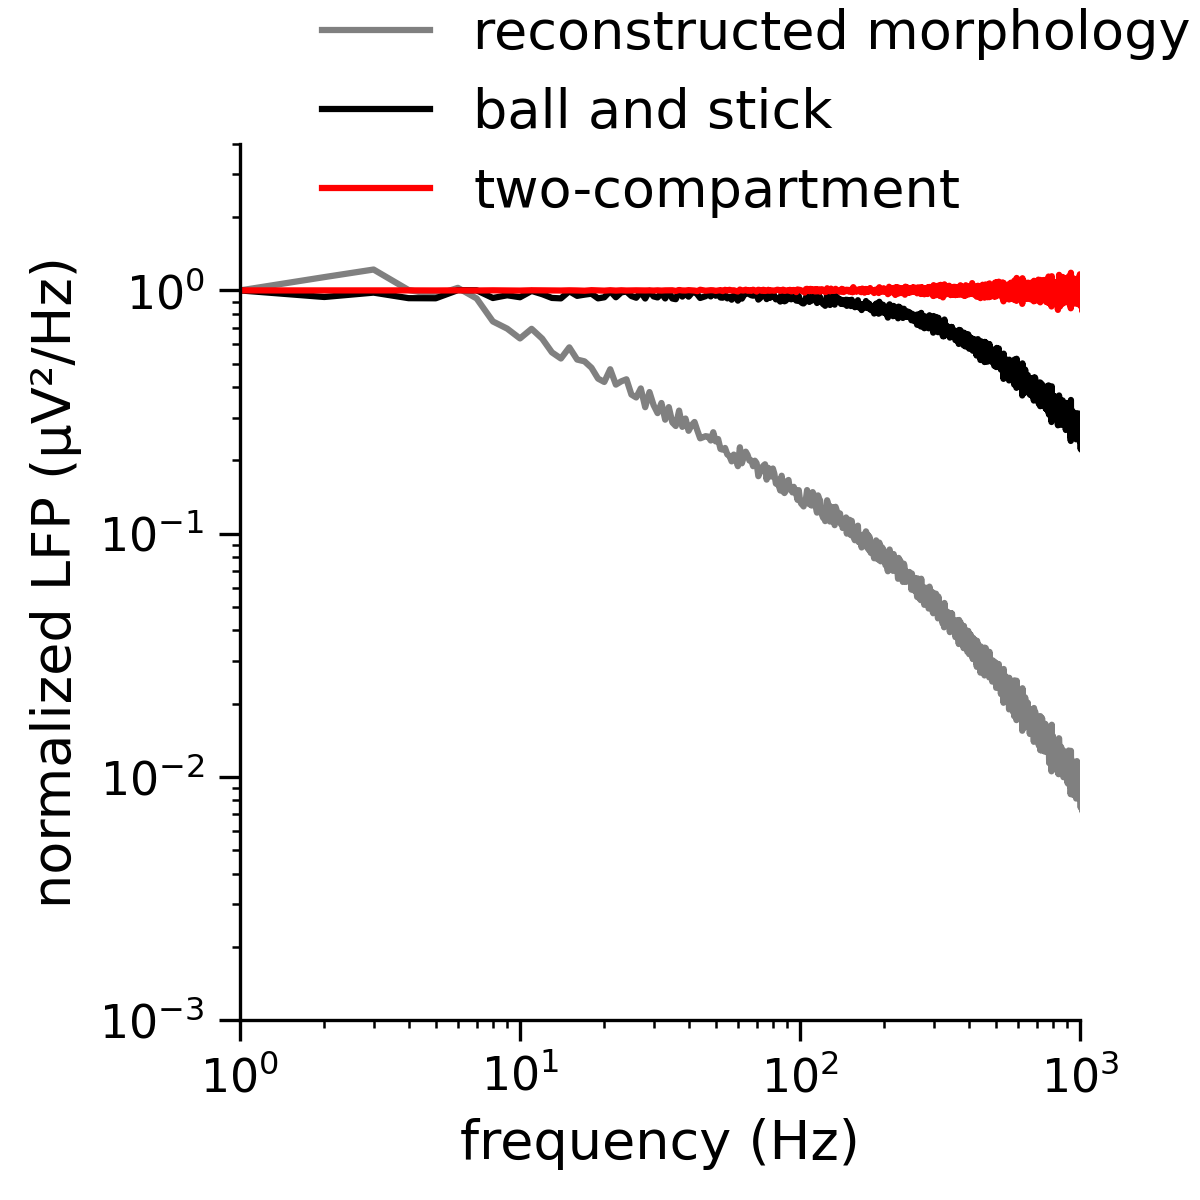
\includegraphics[width=0.4\textwidth]{Figures/LFP/fig_LFP_powerlaws_morphology.png}
\end{center}
\caption{\textbf{The frequency content of the LFP signal is dependent on the morphology.}
White-noise input to soma, measured 200 \si{\micro \metre} away.
}
\label{fig:LFP:morph_matters_PSD}
\end{figure}



\subsection{\red{Intrinsic dendritic filtering}}
\label{subsec:LFP:intrinsic_dend_filt}

An important concept in understanding the origin of LFPs is intrinsic
dendritic filtering \cite**{Linden2010}. This effect causes a low-pass filtering of the LFP with increasing distance from the neuronal sources.
It is caused by the frequency dependence of transmembrane capacitive currents, and it can be illustrated through considering sinusoidal current injection to a simple stick model (\fref{fig:LFP:intrinsic_dendritic_filt}).
From Kirchoff's circuit laws (\fref{chap:Neuron}), we know
that the current injected into a neuronal compartment must equal the current leaving the same compartment, partly through the membrane as a transmembrane current, and partly into other compartments, as axial currents $I_{inj} = I_m + I_a$ (\fref{fig:LFP:intrinsic_dendritic_filt}{\bf A}). We also know that the sum of all transmembrane currents must in this case equal $I_{inj}$, but how much these return currents will be spread out over the membrane of the neuron is dependent on how easy it is for the current to move intracellularly, and how easy it is for the currents to cross the membrane.
The transmembrane current can be expressed as $I_m = c_m\frac{dV}{dt} + I_{ion}$. Note that the transmembrane current is dependent on the time derivative of the membrane potential (through the capacitive current), implying that the membrane is more "leaky" for fast changes in the membrane potential. For a sinusoidal injected current, %$I_{inj} = A \sin (2\pi f t)$,
this means that for increasing frequencies, a larger fraction of the injected current will be balanced by local transmembrane currents instead of axial currents, shifting the transmembrane currents closer to the input site. 
Therefore, rapid changes in the membrane potential are associated with predominately local transmembrane currents, while slow changes in the membrane potential are associated with more distributed transmembrane currents. This can be demonstrated by simulating the extracellular potential around a simple stick model, with a sinusoidal current synapse. A stimulation frequency of 1~Hz gives rise to a large dipolar LFP around the cell, reflecting the distributed nature of the transmembrane currents (\fref{fig:LFP:intrinsic_dendritic_filt}{\bf B}). For the same current amplitude, but with a frequency of 1000~Hz, the resulting LFP is much more spatially confined (\fref{fig:LFP:intrinsic_dendritic_filt}{\bf C}).

This has implications for how the amplitude of different frequency-components will decay with distance from the cell \cite**{Linden2010}. This is because the amplitude of the LFP from a dipole will decay faster in the far-field limit, and the far-field limit is reached at a smaller distance for more spatially confined dipoles \cite**{Linden2010}. In the present example, the amplitude of the LFP very close the the input site was almost identical for the two different frequencies, but the amplitude of the LFP from the high-frequency input decayed more steeply with distance (\fref{fig:LFP:intrinsic_dendritic_filt}{\bf D}). 
For synaptic inputs consisting of both high and low frequency 
components, this means that with increasing distance, the low frequency components will become increasingly dominant in the LFP, causing a low-pass filtering effect in the LFP (\fref{fig:LFP:intrinsic_dendritic_filt}{\bf E}).
Note that this is a quite general result, since we from Fourier analysis know that all signals can be written as a weighted sum of sinusoids with different frequencies.

\begin{figure}[!ht]
\begin{center}
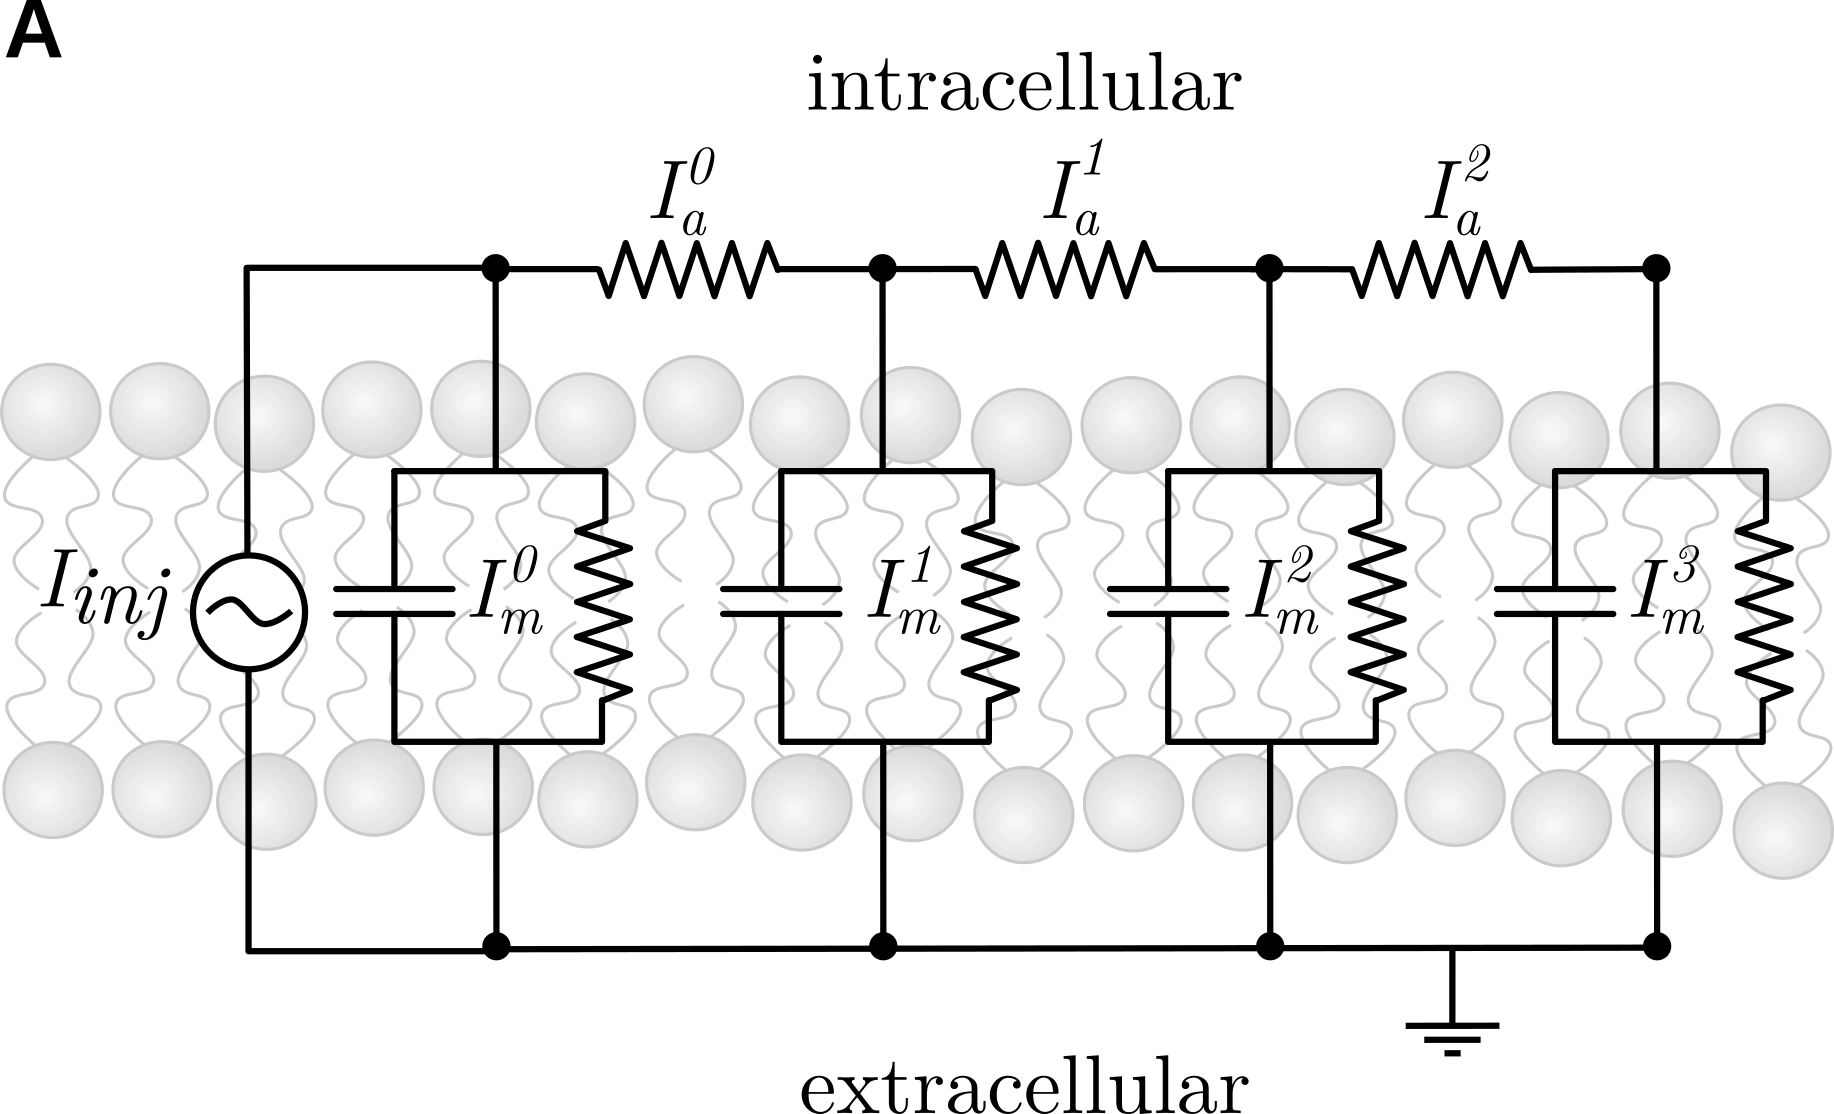
\includegraphics[width=.4\textwidth]{Figures/LFP/cable_equiv_circuit.png}
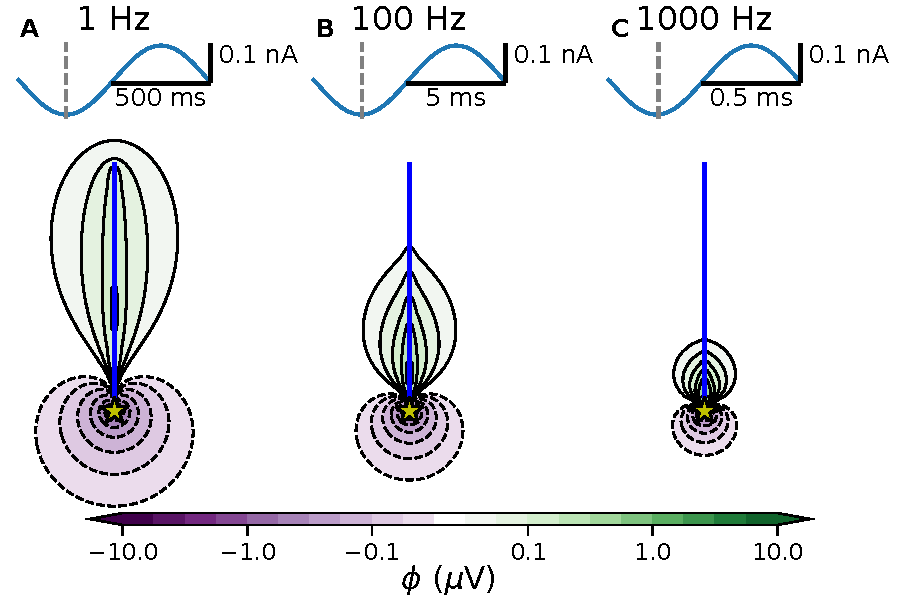
\includegraphics[width=.4\textwidth]{Figures/LFP/intrinsic_dend_filt.pdf}
\end{center}
\caption{\textbf{Intrinsic dendritic filtering.}
Illustration of the LFP at a snapshot in time in response 
to a sinusoidal synapse with different frequencies to a 
dendritic stick.
}
\label{fig:LFP:intrinsic_dendritic_filt}
\end{figure}

Many things affect how much power the LFP has at different frequencies, and different parameters can often affect different frequency regions. The dynamics of the synaptic input mostly affect low-frequency (\fref{fig:LFP:psd_input}).
\begin{figure}[!ht]
\begin{center}
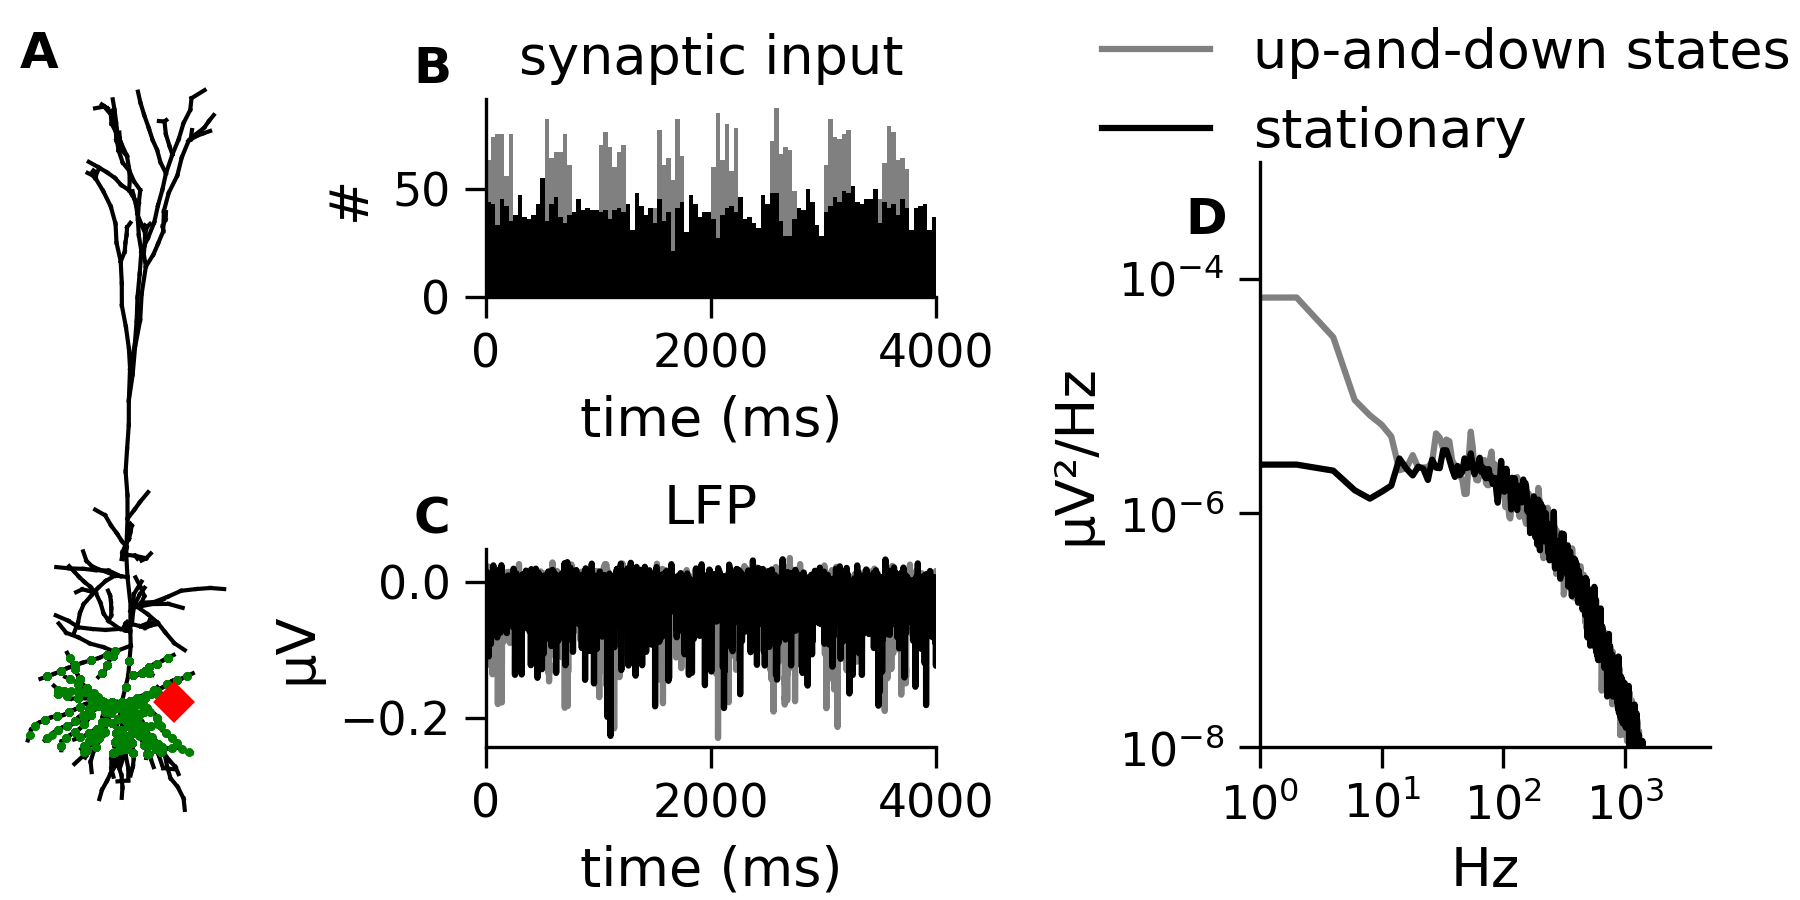
\includegraphics[width=.7\textwidth]{Figures/LFP/fig_LFP_powerlaws_input_dynamics.png}
\end{center}
\caption{\textbf{Frequency-content of LFP signals}
The LFP will have different "power-laws" depending on the parameters. The total number of synaptic inputs is the same in both cases, and all other parameters are identical
\tvnnote{placeholder. Vet ikke om vi skal ha dette. Sammenligne Hay med ball-and-stick og two-compartment?}
}
\label{fig:LFP:psd_input}
\end{figure}



\subsection{\red{TBV:Effect of synaptic correlations}}
It has been demonstrated that correlations in synaptic inputs play a 
vital role in shaping LFP signals, and that receiving correlated synaptic input 
can increase the power of LFP signals from a simulated neural population with orders of magnitude \cite**{Linden2011,Leski2013}. The reason for this can be easily illustrated with a toy example:
We start with a function with a shape slightly reminiscent of a synaptic input (discontinuous jump, followed by exponential decay) (\fref{fig:LFP:correlation_boost}{\bf A}). This function is then added to a much longer "signal" at different specific time points from different "spike trains" (lists of times to insert the function). These spike trains can be constructed to be "uncorrelated" so that each spike train is random and independent, or "correlated", so that each spike train is identical (\fref{fig:LFP:correlation_boost}{\bf B}). If we construct our spike trains so that each spike train has the exact same number of spikes, then necessarily the average value and the area under the curve of the signal will be the same, independent on whether the spike trains are correlated or uncorrelated (\fref{fig:LFP:correlation_boost}{\bf B}). However, if we look at the power spectral density of the signal (or the signal variance), the correlated signal has much more power (higher variance)  (\fref{fig:LFP:correlation_boost}{\bf D}). An intermediate case is when the spike trains are correlated, but a small random "delay" is introduced to the individual spike times (\fref{fig:LFP:correlation_boost}{\bf B}, yellow). This case has the same power as the correlated signal at low frequencies, and the same power as the uncorrelated signal at high frequencies (\fref{fig:LFP:correlation_boost}{\bf D}) (see also \cite**{ElBoustani2009})

\begin{figure}[!ht]
\begin{center}
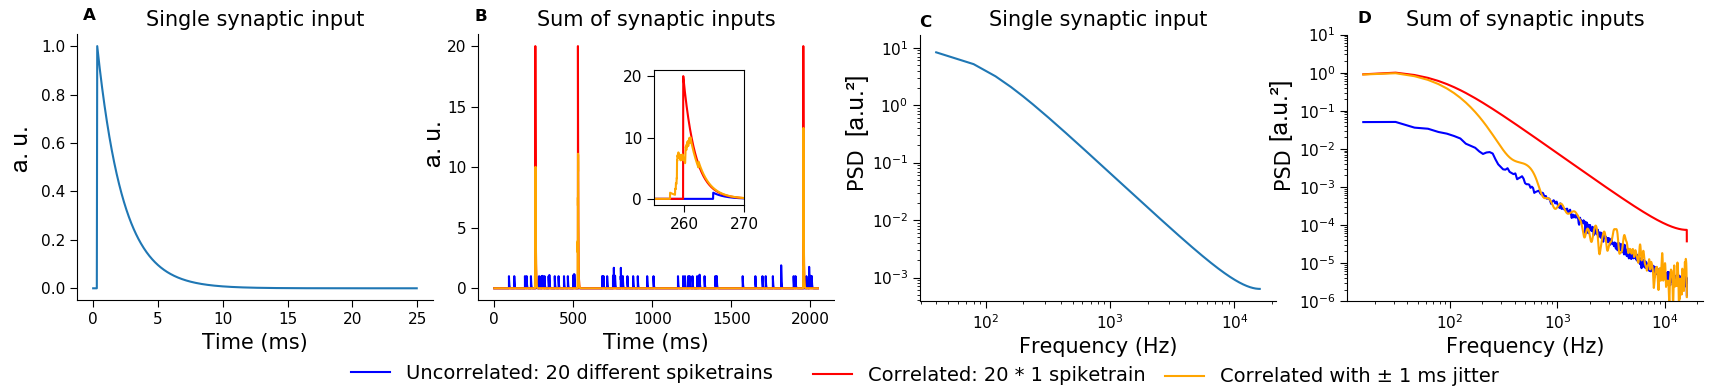
\includegraphics[width=1.\textwidth]{Figures/LFP/LFP_effect_correlation_illustration.png}
\end{center}
\caption{\textbf{Illustration of why correlation in synaptic input boosts LFP.}
Basically, it is just because PSD is squared, and variability increase sum of squares: $(1+3) = (2 +2)$, but $(1^2 + 3^2) > (2^2 + 2^2)$
}
\label{fig:LFP:correlation_boost}
\end{figure}


\subsection{\red{TVN:Effect of spikes on the LFP}}
\tvnnote{Hadde vaert fint aa gaa litt ordentlig igjennom dette, men vi faar se.}
If spikes affect the LFP is not a yes or no question. Depends on many things. Some effect it will be, but maybe not so important
Typically assumed to not be super important. A lot of the spikes are removed by low-pass filter (but see also Fig.~XX).
Amplitude of LFP grows with population size, but spikes are only visible ~30~\si{\micro\metre} away from cell. Observed that LFP fluctuations are much larger, and has a different time course.
\citeasnoun**{Reimann2013} says it is important. Probably is important for hippocampal sharp wave ripples \cite**{Schomburg2012,Luo2018}.
\citeasnoun**{Haider2016} says it is synapses.
Can definitely be expected to contribute somewhat to LFP PSDs.


\subsection{\red{TVN: Effect of subthreshold active conductances}}
Since the LFP is thought to mainly originate from large numbers of synaptic inputs and the resulting return currents, it is reasonable to expect that any ion channel on the cellular membrane that might affect the transmembrane currents, would also affect the LFP. Note that most ion channels are closed at the cells resting potential, and only becomes active during spiking. This is illustrated for a rat layer 5 pyramidal cell model from  \citeasnoun**{Hay2011} in \fref{fig:LFP:subtheshold_linear},
where we see that the simulated somatic membrane potential response to an injected current was almost perfectly linear for a wide range of different subthreshold current amplitudes, and only deviates from this for suprathreshold current input. 

\begin{figure}[!ht]
\begin{center}
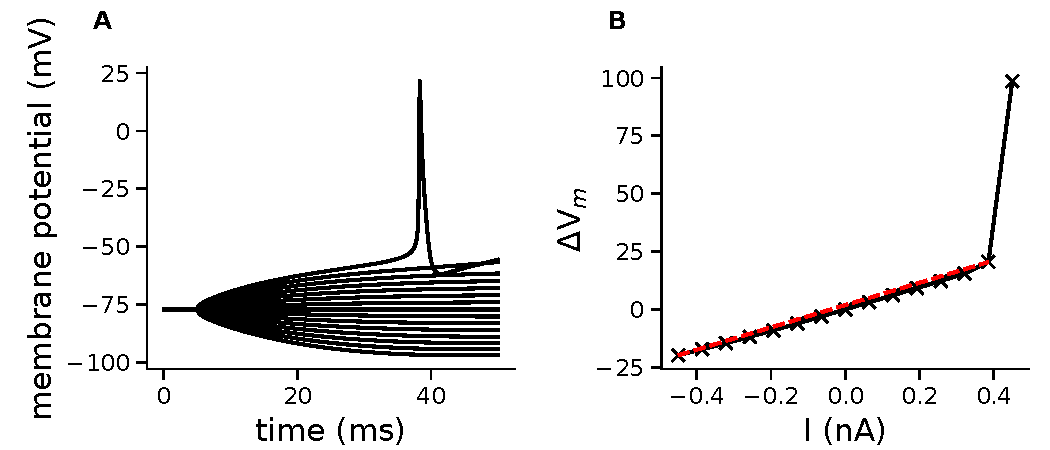
\includegraphics[width=.8\textwidth]{Figures/LFP/fig_hay_subthresh_linearity_test.pdf}
\end{center}
\caption{\textbf{Subthreshold response to somatic current injection is close to linear.}
The somatic membrane potential of the rat pyramidal layer 5 neuron model from cite Hay2011 from exhibits an almost perfectly linear I-V response for somatic subthreshold current injections. Red dashed line is linear.}
\label{fig:LFP:subtheshold_linear}
\end{figure}

There are however certain active conductances that can be expected to affect the LFP, in particular the hyperpolarization-activated cation current $I_{\rm h}$ \index{$I_{\rm h}$}.
In cortical pyramidal cells, the $I_{\rm h}$-conductance is concentrated in the apical dendrite \cite**{Harnett2015,Kalmbach2018}, and for apical synaptic input it was demonstrated in a simulation study to be able to substantially decrease LFP power at frequencies lower than $\sim$30~Hz, causing an apparent resonance peak in the LFP power spectrum \cite**{Ness2016,Ness2018}.

\begin{figure}[!ht]
\begin{center}
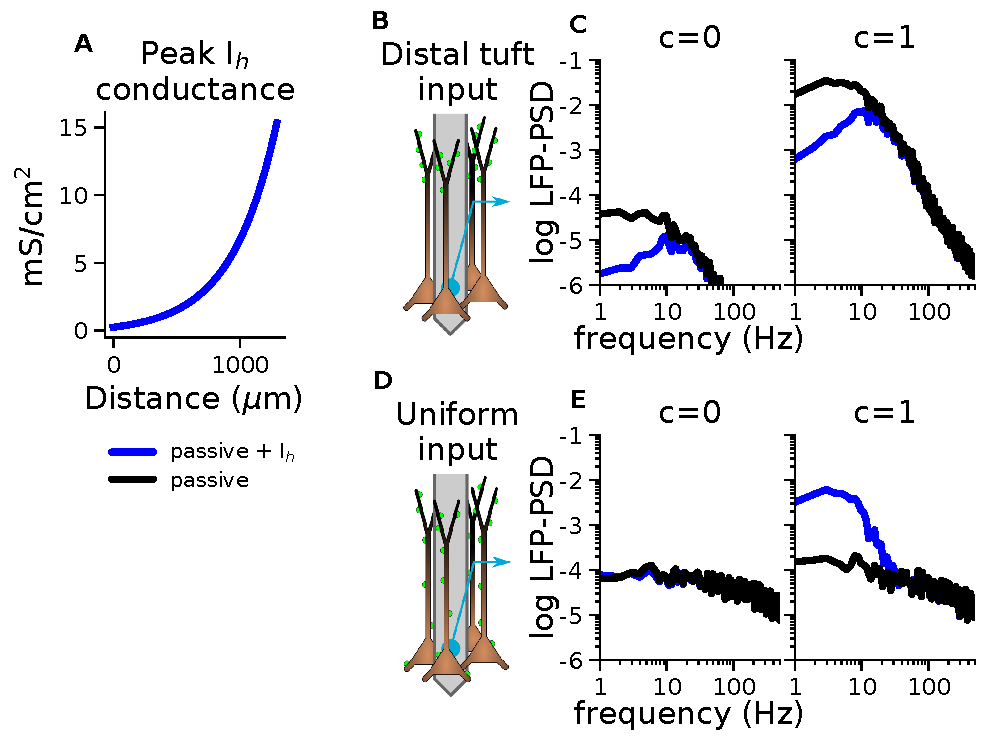
\includegraphics[width=.8\textwidth]{Figures/LFP/effect_of_Ih.pdf}
\end{center}
\caption{\textbf{Affect of Ih on LFP.}
The $I_{\rm h}$-current can affect the LFP.}
\label{fig:LFP:Ih_effect}
\end{figure}

\section{\red{Distance-decay LFP signals from different origins}}
\tvnnote{Lurte litt paa aa ha med litt om hvordan LFP decayer som $1/r^2$ fra enkelt dipol, men $1/r^0$ fra uendelig stort dipol-plan. For eksempel vil LFP signal i L5 kanskje kunne vaere dominert av L23PC hvis en stor nok populasjon der faar input samtidig.}

\section{\red{Unitary LFPs and the kernel method}}
\index{Unitary LFP}
The LFP is mainly generated by the transmembrane currents from synaptic inputs.
We have so far taken what can be called a post-synaptic viewpoint to the LFP, where the single-cell LFP contribution is generated by the synaptic input to the neuron. The total LFP is then the sum of all single-cell contributions. However, we can also take a pre-synaptic viewpoint, where the LFP is generated by all the outgoing synapses of a given neuron. When a neuron spikes, all the outgoing synapses on other neurons are activated (with slightly different delays), meaning that all spike-events are in principle followed by an LFP flash, sometimes referred to as a unitary LFP \cite**{Bazelot2010,Telenczuk2020b}.
Since this approach to the LFP can also include all synaptic events, it is an equivalent way of thinking about the origin of the LFP, 
and in certain cases it can provide new insights.

A single neuron can have thousands of outgoing synapses, but if those synapses are distributed over a large region of the brain, or if the synapses are predominately uniformly distributed over the post-synaptic cells morphology, we can not expect such unitary LFPs to be observable. There are however several examples of where such unitary LFPs can be both measured and modelled.

For example, \citeasnoun**{Swadlow2002} found that the activation of single thalamocortical (TC) neurons, projecting to the somatosensory barrel cortex, gave measurable spike-triggered LFP responses in the somatosensory barrel cortex. These results were later recreated in a modelling study by \citeasnoun**{Hagen2017}.

In hippocampus, \citeasnoun**{Bazelot2010} demonstrated that unitary LFPs could be recorded from interneurons, but not from pyramidal neurons.
 
Initially, this mights seem at odds with earlier claims that 
the LFP is generated by pyramidal neurons, but
these claims are in fact perfectly compatible: The LFP itself is generated by transmembrane currents in pyramidal neurons, but it can still be dominated by the synaptic input from inhibitory neurons. In other words, if we take the post-synaptic viewpoint we would say that the LFP is dominated by synaptic input to pyramidal cells, while if we take the pre-synaptic viewpoint, we would say that the LFP is (at least in some cases) dominated by the synaptic output of inhibitory neurons \cite**{Bazelot2010,Hagen2016,Telenczuk2017,Telenczuk2020b}.

 If 
 distributed over a large region, and therefore such post-spike LFP flashes can be expected to be cover a large region, but be very weak everywhere. They can be measured \cite**{Swadlow2002,Bazelot2010,Telenczuk2017}, and modelled \cite**{Hagen2017,Telenczuk2020a,Telenczuk2020b}.

Kernel method for populations: Populations: \cite**{Hagen2016,Skaar2020,Telenczuk2020a}
\index{Kernel method}

\section{\red{Current Source Density (CSD) analysis}}
LFPs are only interesting in that they might reveal something
about the underlying neural activity.
Therefore, LFPs are often analysed in terms of the the CSD,
since this is better linked to the underlying neural activity.
iCSD is better than CSD.
Problem of ground/baseline goes away for CSDs.
\tvnnote{Hva skal vi ha med her?}

\section{\red{Validation of framework}}
\tvnnote{Jeg foeler vi typisk skriver "LFP is thought to mainly reflect synaptic input", og sleger paa en sitering til en kilde som vel egentlig bare sier akkurat det samme.
 Jeg har lyst til aa dedikere litt plass til
"validering". Type: Hvilke beviser finnes for at LFP i hovedsak stammer fra synaptisk input?
Jeg tror dette er paa sin plass, i og med at vi alltid uttrykker en viss usikkerhet angaaende opphavet til LFP, det er hvertfall litt kontroversielt, og vi paapeker at LFP er vanskelig aa tolke.
Kan muligens flette dette inn i introduksjonen til LFP?
}

What evidence do we have that measured LFP signals mostly reflect synaptic input to populations of neurons?
It is well-established that changes in synaptic weights (plasticity) are reflected in the LFP amplitude, and for example long-term potentiation (LTP) was first discovered by changes in the LFP amplitude \cite**{Bliss1973}.

Laminar distribution makes sense, and L4 has MUA but initially little LFP, as expected

The time-course of LFP signals are perfectly in line with expectations from synapses, and synaptic input times.

We lack any other reasonable candidate: Spikes can certainly be expected to contribute somewhat, but can not account for observed LFPs.

Mono-synaptic unitary LFPs: First spike, then LFP \cite**{Swadlow2002,Bazelot2010}, is perfectly in sync with modelling \cite**{Hagen2017,Telenczuk2020b}.


\section{\red{TVN: Other approaches}}

\begin{itemize}
\item "Magic" simple formula \cite**{Mazzoni2015}
\item Kernel trick \cite**{Hagen2016,Skaar2020}
\end{itemize}

\subsection{\red{TBV:Population LFPs}}
\begin{itemize}
\item Full simulations \cite**{Linden2011,Leski2013}
\item Analytical results \cite**{Einevoll2013a}
\item Active dendrites \cite**{Ness2018}
\item Effect of correlations
\end{itemize}




\section{\orange{GTE: Example: How local is the  local field potential?}}
\label{LFP:sec:how-local-is-the-local-field-potential}

The recording of LFPs has a long history in neuroscience. Therefore maybe it is surprising that the question 
`How local is the local field potential' is still debated. How many neurons contribute to the LFP 
recorded by an electric contact? Alternatively, what is the typical radius of the volume surrounding the contact containing
the neurons generating (almost) all of the recorded LFP,  referred to as the \index{spatial reach}? 
Experimental answers to this question have been conflicting, giving estimates for the spatial reach spanning from
a few hundred micrometers~\cite**{Katzner2009,Xing2009} to several millimetres~\cite**{Kreiman2006} or more~\cite**{Kajikawa2011}.
Modelling has revealed that these experimental observations can be reconciled, the key finding being that the spatial reach depends strongly
on how synchronous the synaptic inputs driving the LFP-generating neurons are~\cite**{Linden2011}.

%In \citeasnoun**{Linden2011} it was found that the spatial
%reach depends strongly on how synchronous the synaptic inputs driving the LFP-generating neurons are, see 
%Box~\ref{mm:box:how-local-is-the-local-field-potential}. When the synaptic inputs
%impinging on the population are asynchronous, that is, \firstterm{uncorrelated}, the spatial reach can be as low as hundred micrometers. However, when the synaptic inputs are synchronous manner, that is, \firstterm{correlated}, the spatial reach can be millimetres and even centimeters. 

In \citeasnoun**{Linden2011} this question was addressed by calculationg the spatial size of the pool of neurons 
contributing to the LFP recorded by an electrode. The model used to explore this question
is shown in panel (a) in Figure~\ref{LFP:fig:how-local}.
Here a population of identical pyramidal neurons receiving synaptic inputs is positioned
with circular symmetry in a disc around the recording electrode. The LFP contributions from the individual neurons 
$\phi_i(t)$ sum up to give the total population LFP  $\phi(t)$ (panel b).

%%%%%%%%%%
% Figure: LFP - how local is the local field potential 
%%%%%%%%%%
%\begin{cnfigure}{Figures/mm/how-local-is-the-LFP-w90-r150}
\begin{figure}
\begin{center}
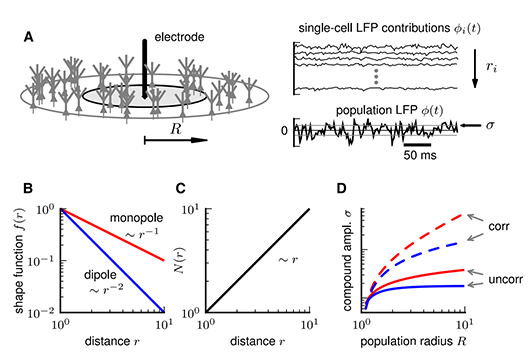
\includegraphics{Figures/LFP/LFP-how-local-is-the-LFP-w90-r150}
\end{center}
\caption[]{Illustration of modelling approach used to explore the question
about the extent of the local field potential.
\gen{The "monopole" part of the figure will not be included.}
\gen{Figure and caption to be updated.}
}
\label{LFP:fig:how-local}
%\figpermOurs
\end{figure}
%%%%%%%%%%%%%%%%%%
  
This total population LFP signal can be computed by using 
Equation~\ref{XX:equation:Ve-multi-compartment} to first compute the signal contribution from each neuron and 
then sum up all the single-neuron contributions to get the compound LFP from the entire population of neurons.
With increasing radius $R$ of the population, more and more neurons will contribute to the compound LFP $\phi(t)$,
and the amplitude $\sigma(R)$ (Figure~\ref{LFP:fig:how-local}b) is thus expected to increase with
$R$. On the other hand the contribution to the compound signal from a single neuron decreases with distance 
as seen in Section~\ref{XX:sec:LFP-single-neurons}, and so intuitively one could expect that $\sigma(R)$ approaches
a constant value $\sigma_\infty$ as the population size $R$ increases. One can then define the spatial reach as the radius for which
the compound LFP has reached a certain fraction $\alpha$ (for example $\alpha$=0.95 as in \citeasnoun**{Linden2011}) of this limiting value $\sigma_\infty$. 

However, it is not clear at the outset that $\sigma(R)$ converges towards a fixed value as $R$ increases and that
a spatial reach defined in this way exists. It turns out that a finite spatial reach is obtained under some conditions, but not all.
We next consider a simple qualitative model that illuminates what factors determine $\sigma(R)$ and when the conditions for
which it converges to a finite value as $R$ increases. 

\subsection{\orange{GTE: Qualitative model}}
Two factors are expected to be key in determining how the compound population LFP $\sigma(R)$ increases with $R$:
(i) how sharply the single-neuron contribution, that is, the \index{shape function} $f(r)$, decays with distance from the neurons, and (ii) the number
density $N(r)$ of neurons positioned in a ring of radius $r$ around the electrode. Here we are interested in the compound LFP for large values of
$R$, and for this only the behavior of the shape function $f(r)$ far away from the neuron is of interest. For such large distances, the far-field dipole approximation
can be assumed, that is, $f(r) \propto 1/r^2$ (Figure~\ref{LFP:fig:how-local}c). 
The number of neurons within each ring will be proportional to the circumference $2\pi r$
of the ring, and $N(r)$ will thus be proportional to $r$ (panel d).

A third key factor is the level of \index{correlations} between the single-neuron contributions to the compound LFP. 

\subsubsection{Uncorrelated single-neuron LFPs}
%\paragraph{Uncorrelated single-neuron LFPs}
In a situation
where the neurons in the population each receive synaptic inputs at completely random times, the contributions will be \index{uncorrelated}, and
there will be strong cancellations of the individual LFP contributions. In this case, the amplitude of the compound signal  $\sigma(R)$ will not be proportional 
to the number of individual sources. However, the variance of the compound LFP, that is, the square of  $\sigma(R)$, will be
given as the sum of the variances of the individual single-neuron contributions. 
(This is analogous to the situation with a so-called random walker where
the variance, that is, square, of the displacement of the walker after $N$ random kicks is proportional to $N$, see, for example, \citeasnoun[Ch. X]{nelson2008}.)

In this case one expects \cite**{Linden2011}
%%%
\begin{equation}
\sigma_\text{u}(R)^2 \propto \sum_i \sigma_i^2 \propto \sum_i f(r_i)^2
\label{LFP:equation:sigmaR2-uncorrelated-sum}
\end{equation}
%%%
Here $\sigma_i$ represents the amplitude of the LFP contribution from the single 
neuron $i$ (Figure~\ref{LFP:fig:how-local}b). This contribution is assumed to 
be proportional to the shape function $f(r_i)$ where $r_i$ is the distance from neuron $i$ to the recording electrode.  
We have further added the subscript `u' to denote that this formula applies to the case of uncorrelated single-neuron LFP contributions.

With many neurons contributing to the compound LFP, we can approximate the sum in Equation~\ref{LFP:equation:sigmaR2-uncorrelated-sum}
with the integral  
%%%
\begin{equation}
\sigma_\text{u}(R)^2 \propto \int_0^R N(r) f(r)^2 dr 
\label{LFP:equation:sigmaR2-uncorrelated-integral}
\end{equation}
%%%
The present focus is on the contribution from the distant neurons where the far-field limit of $f(r)$ applies, that is, where $f(r) \propto 1/r^2$.
For the contributions from these neurons we can approximate the integral in Equation~\ref{LFP:equation:sigmaR2-uncorrelated-integral}
with 
%%%
\begin{equation}
\sigma_\text{u}(R)^2 \sim \int_{R_x}^R N(r) \left(\frac{1}{r^2}\right)^2 dr \propto \int_{R_x}^R \frac{1}{r^3} dr
\propto \frac{1}{R_x^2}-\frac{1}{R^2}
\label{LFP:equation:sigmaR2-uncorrelated-integral-2}
\end{equation}
%%%
Here we have for convenience introduced a lower cut-off radius $R_x$ in the integral to remove the unphysical divergence that would appear by
assuming the far-field relationship $f(r)\sim 1/r^2$ for distances $r$ approaching zero.

The key observation from Equation~\ref{LFP:equation:sigmaR2-uncorrelated-integral-2} is that the variance $\sigma_\text{u}(R)^2$ 
will approach a fixed finite value $\sigma_\infty$ as $R \rightarrow \infty$ (since $1/R^2 \rightarrow 0$ in this limit), Figure~\ref{LFP:fig:how-local}d.
This in turn implies that a spatial reach corresponding to the value of $R$ for which $\sigma_\text{u}(R)=\alpha \sigma_\infty$ can be found.
In the quantitative modelling below, we will see that this spatial reach roughly corresponds to the lateral extension of the dendritic bush, that is, a few hundred micrometers or so when a value of $\alpha$ close to unity is chosen.

\subsubsection{Correlated single-neuron LFPs}
%\paragraph{Correlated single-neuron LFPs}

For fully correlated synaptic inputs onto the neurons, the single-neuron LFP contributions to the compound population LFP will overlap in time.
Further, if the different synaptic inputs have similar spatial positions on the receiving neurons, for example, all placed on the apical dendrites,  there will be little cancellation of their contributions of the single-neuron LFP contributions. 
This is akin to constructive interference in wave physics when, for example, water waves from several sources are added to give interference patterns and a summation of wave crests from the individual wave sources sum up to give a large compound wave.

In this case the compound LFP can be 
approximated by simply summing the individual amplitude contributions. Formulated as an integral, this gives
%%%
\begin{equation}
\sigma_\text{c}(R) \propto \int_0^R N(r) f(r) dr 
\label{LFP:equation:sigmaR-correlated-integral}
\end{equation}
%%%
When we now insert $N(r) \sim r$ and $f(r) \sim 1/r^2$, we find that the contributions from the neurons
positioned outside a radial distance $R_x$ from the electrode is given by
%%%
\begin{equation}
\sigma_\text{c}(R) \propto \int_{R_x}^R r \frac{1}{r^2} dr =  \int_{R_x}^R \frac{1}{r} dr = \ln \frac{R}{R_x} 
\label{LFP:equation:sigmaR-correlated-integral-2}
\end{equation}
%%%
The key observation here is that the amplitude $\sigma (R) \rightarrow \infty$ when $R \rightarrow \infty$.
Thus unlike for the uncorrelated case, the LFP amplitude increases without bound as the population size $R$ increases, 
and the compound LFP signal thus has an `infinite' spatial reach.

The question of whether the spatial reach of the LFP signal is finite or infinite has some resemblance to  
the ancient question of why the night sky is dark given the numerous stars in the universe. This so-called
Olbers' paradox and the link to the spatial-reach question is described in Box XX.


\subsection{\red{GTE: Box:  Why is the night sky dark? Olbers' paradox}}
\gen{Was a Box in chapter in Sterratt}
%%%%%%%%%%
% Box: Why is the night sky dark? Olbers' paradox
%%%%%%%%%%
%\begin{boxfloat}{Olbers' paradox and population LFPs}
%  \label{LFP:box:Olbers}
%
\begin{center}

\includegraphics{Figures/LFP/LFP-night-sky-w90-r150}
\end{center}
\vspace*{6pt}
%
Why is the night sky dark? An interesting historical paradox from astronomy, known as Olbers' paradox~\cite**{Harrison1989}, has some analogies with the question of summation of LFP signals from many neurons. The question is why the night sky is dark given the following:
(i) the light intensity from a single star falls off as $1/r^2$, (ii) in a homogeneous universe the number of stars in a spherical shell of a certain thickness around the Earth should increase as $r^2$. According to this the contribution from each such shell of stars to the illumination on Earth should thus be independent of the distance $r$. With an infinite universe there will be an infinite number of shells and thus an infinite light intensity on Earth! This paradox is resolved if one takes into account modern knowledge that the universe is not infinitely old and the speed of light is finite so that there are no contributing stars for shells at distances of 14 billion light years or more away. This summation of light from numerous starts is analogous to the summation of LFP from numerous neurons in the surrounding brain. A difference is that while neuronal LFPs are essentially dipoles, the stars are monopole light sources. Also the geometry is different (three-dimensional shells for stars, two-dimensional rings for neurons). The outcome is that while a finite brain is not required for a finite LFP, a finite universe is indeed required to resolve Olbers' paradox.
\gen{This text is copied directly from a book chapter we wrote (Einevoll2013a) and should be modified to avoid self-duplication.}
%\end{boxfloat}
%%%

\subsection{\orange{GTE: Quantitative model}}

The results from the qualitative modelling above demonstrates that the size of the compound LFP 
from a population of neurons receiving synaptic inputs, depend critically on the level of 
correlation in the synaptic inputs. To obtain a more
precise picture of how the compound LFP grows with population size, we here investigate a 
corresponding quantitative model where the single-neuron contributions $f(r)$ is specified in detail.

Figure~\ref{LFP:fig:how-local-shape-function} shows results for how the LFP signal decays with distance from the soma of neurons when moving sideways from the depth of the neuronal somas
(similar to  Figure~\ref{LFP:fig:distance-decay}c). As seen in Figure~\ref{LFP:fig:how-local-shape-function}b, the decay of the LFP signal with lateral distance follows a very standardised form. For all three neuronal morphologies considered the single-neuron LFP signal decays roughly as $1/\sqrt{r}$ close to the neuron and as $1/r^2$ (as expected for a current dipole) far away from the neuron. 

This suggests the following general form for the shape function $f(r)$ 
(Figure~\ref{LFP:fig:how-local-shape-function}c,d):
%
\begin{equation}
  f(r)=
  \begin{cases}
    f_0 & r< r_\varepsilon \\
    f_0\,\left(r_\varepsilon/r\right)^{1/2} &  r_\varepsilon \le r < r_* \\
    f_0\,\left(r_\varepsilon/r_*\right)^{1/2}\,\left(r_*/r\right)^{2}  & r \ge r_* \;\;,
  \end{cases}
\label{LFP:equation:f-power-law}
\end{equation}
%
Here $r_*$ is the radial distance at which the amplitude decay changes from $1/\sqrt{r}$ to $1/r^2$.
From Figure~\ref{LFP:fig:how-local-shape-function}b we see that $r_*$ is about 100~micrometers for all the presently considered neurons. We have also introduced a lower cut-off $r_\varepsilon$ under 
which the signal is assumed to be constant rather than diverging as $1/\sqrt{r}$. This cut-off reflects the finite size of the neuronal somas so $r_\varepsilon$ could be about 10 micrometers or so. 

For the example in Figure~\ref{LFP:fig:how-local-shape-function} where synaptic inputs are evenly spread across the dendritic membranes, the parameter $r_*$ can be assumed to be roughly the same for the three example neurons. This is not so for the parameter $f_0$ describing the overall amplitude of the signal, however. This parameter will in general depend not only on the neuronal morphology, but in particular on the number and strength of synaptic inputs ~\cite**{Linden2010,Linden2011,Einevoll2013a}.

%%%%%%%%%%
% Figure: LFP - how local - shape - function
%%%%%%%%%%
%\begin{cnfigure}{Figures/mm/EP-how-local-shape-function-w100-r150}
\begin{figure}
\begin{center}
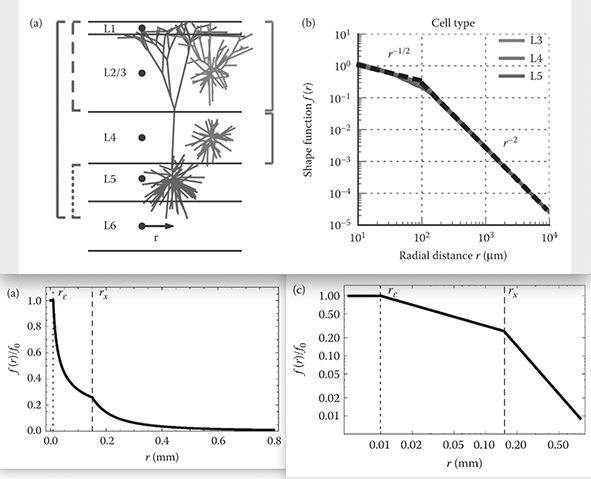
\includegraphics{Figures/LFP/LFP-how-local-shape-function-w100-r150}
\end{center}
\caption[]{Shape function
\gen{Figure and caption to be updated.Change $r_*$ to 0.1 mm?
Mention uncorrelated inputs to make figure. Mention that $r_*$ is larger for apical inputs
onto L5 neurons, cf. Figure in Linden 2011.}
}
\label{LFP:fig:how-local-shape-function}
%\figpermOurs
\end{figure}
%%%%%%%%%%%%%%%%%%


\subsubsection{Uncorrelated single-neuron LFPs}
%\paragraph{Uncorrelated single-neuron LFPs}

For the case with uncorrelated single-neuron LFPs, the integral in Equation~\ref{LFP:equation:sigmaR2-uncorrelated-integral} for the variance of the compound LFP signal can now
be written as 
%%%
\begin{equation}
\sigma_\text{u}(R)^2  = \int_0^R N(r)  f(r)^2 dr  = \rho \int_0^R 2 \pi r  f(r)^2 dr 
\label{LFP:equation:sigmaR2-uncorrelated-quantitative}
\end{equation}
%%%
where we have used $N(r)dr=2\pi r \rho dr$ with $\rho$ being the area density of neurons
contributing to the LFP. Insertion of $f(r)$ from 
Equation~\ref{LFP:fig:how-local-shape-function} then gives after some algebra
%%%
\begin{equation}
  \sigma_\text{u}(R)^2= 
  \begin{cases}
    f_0^2 \, \rho \, \pi R^2                   &   R \le r_\varepsilon   \;\;,\\
    f_0^2 \, \rho \, \pi r_\varepsilon (2 R - r_\varepsilon)  &   r_\varepsilon \le R \le r_*  \;\;,\\
    f_0^2 \, \rho \, \pi r_\varepsilon (3 r_* - r_\varepsilon  - r_\star^3/R^2)  & R \ge r_* \;\;,
  \end{cases}
\label{LFP:equation:sigmaR2-uncorrelated-quantitative-2}  
\end{equation}
%%%
The corresponding formula for the LFP amplitude $\sigma_\text{u}(R)$, found by taking the 
square root of the expressions in Equation~\ref{LFP:equation:sigmaR2-uncorrelated-quantitative-2},
is illustrated in Figure~\ref{LFP:fig:how-local-center-of-population}(a).  
\gen{ Unsure whether to give the formula for $\sigma_\text{u}(R)$ instead of $\sigma_\text{u}(R)^2$.}

%
%%%%%%%%%%
% Figure: LFP - how local - center of population
%%%%%%%%%%
%\begin{cnfigure}{Figures/mm/EP-how-local-center-of-population-w100-r150}
\begin{figure}
\begin{center}
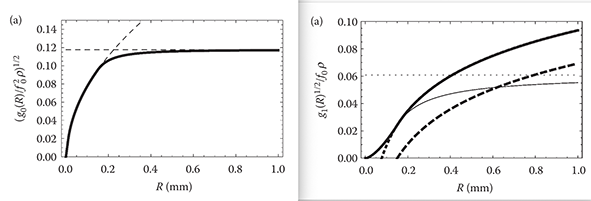
\includegraphics{Figures/LFP/LFP-how-local-center-of-population-w100-r150}
\end{center}
\caption[]{Population LFP at center of population for uncorrelated neurons.
\gen{Figure and caption to be updated. 
Panel (a) must include region smaller than $r_\varepsilon$. Explain dashed lines.
Change $r_*$ to 0.1 mm? Make figure with real numbers (millivolts) on the y-axis.}
}
\label{LFP:fig:how-local-center-of-population}
%\figpermOurs
\end{figure}
%%%%%%%%%%%%%%%%%%
%

A first observation from the figure is that $\sigma_\text{u}(R)$ seems to approach a finite
value as $R \rightarrow \infty$, and from the formula in Equation~\ref{LFP:equation:sigmaR2-uncorrelated-quantitative-2}  
we see that this value is given by $\sigma_\infty = f_0^2 \, \rho \, \pi r_\varepsilon (3 r_* - r_\varepsilon)$. For the parameter values used in Figure~\ref{LFP:fig:how-local-center-of-population} this gives  
$\sigma_\infty=$XX~millivolts. 

The analytical formulae in Equation~\ref{LFP:equation:sigmaR2-uncorrelated-quantitative-2} 
further suggest a new definition of the spatial reach $R_\text{reach}$, that is, $R_\text{reach}$ 
can be set to be the distance from the electrode at which the 
intermediate-$R$ ($r_\varepsilon \le R \le r_*$) and the 
infinite-$R$ ($R \rightarrow \infty$) formulae intersect~\cite**{Einevoll2013a}, see 
Figure~\ref{LFP:fig:how-local-center-of-population}a. For this particular value of $R$ we have 
$2R_\text{reach}-r_\varepsilon=3 r_* - r_\varepsilon$, that is, $R_\text{reach} =1.5 r_*$. 

Insertion of $R=R_\text{reach}=1.5 r_*$ into Equation~\ref{LFP:equation:sigmaR2-uncorrelated-quantitative-2} 
gives that $\sigma (R_\text{reach})=\sqrt{23/27}\sigma_\infty \simeq 0.92 \sigma_\infty$ independent of the value of $r_*$ (as long as $r_\varepsilon \ll r_*$ like it is in the present numerical example). Thus for the present case with uncorrelated neuronal sources, the model implies that 92\% of the LFP amplitude recorded by an electrode in the centre of a disc-like population 
stems from neurons closer than $R_\text{reach}=1.5~r_*$. For the numerical values
used in Figure~\ref{LFP:fig:how-local-center-of-population}a,
this corresponds to $R_\text{reach}$=0.15~mm. 
Note that this result pertains to the situation where the electrode is at the same depth level as the neuronal somas. But the same reasoning and modelling can equally be used for the case where the neuronal somas are above or below the recording electrode, see~\citeasnoun**{Einevoll2013a}.

We can now ask the question of how many neurons contribute to the recorded LFP. To get a rough idea, we can estimate the number of neurons with somas contained within a sphere of radius $R_\text{reach}$
around the electrode. With a neuron density of, for example, $\rho_\text{neuron}$=50000 neurons per mm$^3$ which is typical for grey matter in 
cortex~\gen{REF:Beaulieu 1993}, we find that this sphere will contain $N_\text{neuron}=4 \pi R_\text{reach}^3 \rho_\text{neuron}/3$=\gex{XX}~neurons.


\subsubsection{Correlated single-neuron LFPs}
%\paragraph{Correlated single-neuron LFPs}

For the case with correlated single-neuron LFPs, insertion of the shape function $f(r)$ from 
Equation~\ref{LFP:equation:sigmaR2-uncorrelated-quantitative-2}  into the integral
%%%
\begin{equation}
\sigma_\text{c}(R)  = \int_0^R N(r)  f(r) dr  = \rho \int_0^R 2 \pi r  f(r) dr 
\label{LFP:equation:sigmaR2-correlated-quantitative}
\end{equation}
%%%
gives
%%%
\begin{equation}
  \sigma_\text{c}(R) =
  \begin{cases}
    f_0^2 \, \rho^2 \, \pi^2 R^4                   &   R \le r_\varepsilon   \;\;,\\
    f_0^2 \, \rho^2 \frac{1}{9} \pi^2 \left( r_\varepsilon^2 - 4 r_\varepsilon^{1/2} R^{3/2} \right)^2 \;\;, &   r_\varepsilon \le R \le r_* \\
    f_0^2 \, \rho^2 \frac{1}{9} \pi ^2 r_{\varepsilon } \left(r_{\varepsilon }^{3/2}-\left(4+6 \ln\left(R/r_*\right)\right) r_*^{3/2}\right)^2
  & R \ge r_* \;\;,
  \end{cases} 
  \label{LFP:equation:sigmaR2-correlated-quantitative-2}  
\end{equation}
%%%
In this case the compound population LFP amplitude $\sigma_\text{c}(R)$ does not approach a finite fixed value $\sigma_\infty$ as $R \rightarrow \infty$, rather the LFP amplitude
displays logarithmic divergence, i.e., $\sigma (R) \sim \ln(R/r_*)^2$ in this limit, see Figure~\ref{LFP:fig:how-local-center-of-population}b.
Thus the LFP would in principle be infinite if the electrode was surrounded by an infinite sea of correlated neuronal LFP sources. Of course, this unbounded amplification of the LFP amplitude will never occur  
due to the necessarily finite size of pools of correlated neuronal LFP sources in the cortex. (In fact, this is also an explanation for 
why the night sky is dark and not light due to the illumination from all the stars surrounding us, see  Box \gex{Olbers}.
%~\ref{LFP:box:Olbers}.)

For correlated LFP sources, the model predicts that the spatial reach in practice will be set by the size of the pool of neurons receiving correlated synaptic inputs surrounding the electrode, see \citeasnoun[Figure~5]{Linden2011}. This may explain why experimental estimates of the spatial reach has varied so widely, from a few hundred micrometers to centimetres \gen{Kreiman2006, Liu and Newsome2006, Berens et al 2008a, Katzner2009, Xing et al. 2009}.

The above formulae for $\sigma_\text{c}(R)$ for the population LFP represent the two extreme cases where either the single-neuron
LFPs are completely uncorrelated (Equation~\ref{LFP:equation:sigmaR2-uncorrelated-quantitative-2}) or completely correlated 
(Equation~\ref{LFP:equation:sigmaR2-correlated-quantitative-2}). In reality one would expect the situation to be somewhere in between, that is,
the single-neuron LFPs will be partially correlated. However, a corresponding formula for $\sigma_\text{c}(R)$ for arbitrarily levels of correlations can also be found, see Box~\ref{LFP:box:population-LFP-general}. 

\gen{GTE: Note that the boost of LFPs requires asymmetric input.}
 
 
 
%%%%%%%%%%
% Box: General expression for compound LFP
%%%%%%%%%%
\subsection{\red{GTE: Box: General expression for population LFP}}
\gen{This was a box in Sterratt chapter}
%\begin{boxfloat}{General expression for population LFP}
%  \label{LFP:box:population-LFP-general}
The formulae in Equations~\ref{LFP:equation:sigmaR2-uncorrelated-quantitative-2} 
and~\ref{LFP:equation:sigmaR2-correlated-quantitative-2} predict how the amplitude  $\sigma$ 
for the population LFP will depend on the population radius $R$ for the cases of uncorrelated or completely correlated
single-neuron LFPs, respectively. However, an analogous formula for the intermediate case with partially correlated single-neuron LFPs, can
also be derived.

Following \citeasnoun**{Linden2011} we assume the single-neuron LFP contribution $\phi_i(t)$ from a neuron $i$ to be a product of a 
temporal part $\xi_i(t)$ and a spatial part $f(r_i)$ where $r_i$ is the distance between the neuron and the electrode:
%%%
\begin{equation}  
\phi_i(t)= \xi_i(t) f(r_i)
\label{LFP:box:equation:phii}
\end{equation}
%%%
Further, $f(r_i)$ is assumed to be given by the shape function in 
Equation~\ref{LFP:equation:f-power-law}, and $\xi_i(t)$ is a time-dependent function with a mean value of zero and a unit variance, that is,
$\langle \xi_i(t)^2 \rangle$=1. Here $\langle \cdot \rangle$ represents averaging over time.

We now introduce the \index{pair-wise correlation} 
%%%
\begin{equation}
c_\phi=\langle \xi_i(t) \xi_j(t)\rangle\, ,\;\; i \neq j
\label{LFP:box:equation:phii}
\end{equation}
%%%
and assume that is has the same value for all pairs $i \neq j$. With this notation,  
\emph{uncorrelated} single-neuron LFP sources corresponds to $c_\phi=0$ and 
completely \emph{correlated} single-neuron LFP sources corresponds to $c_\phi=1$.

With the general applicable expression
%%%
\begin{equation}
\langle \phi_i(t) \phi_j(t) \rangle= c_\phi f(r_i) f(r_j)\, , \;\; i \neq j
\label{LFP:box:equation:phii-phij}
\end{equation}
%%%
it was shown in \citeasnoun**{Linden2011} that the population LFP amplitude is given as
%%%
\begin{equation}
  \sigma(R)=\sqrt{(1-c_\phi) \sigma_\text{u}(R)^2 +  c_\phi \sigma_\text{c}(R)^2}\;\;.
  \label{LFP:box:equation:sigmaR}
\end{equation}
%%%
where $\sigma_\text{u}(R)$ is given by the expression in Equation~\ref{LFP:equation:sigmaR2-uncorrelated-quantitative-2} and
 $\sigma_\text{c}(R)$ by the expression in Equation~\ref{LFP:equation:sigmaR2-correlated-quantitative-2}.

A notable difference between the uncorrelated $\sigma_\text{u}(R)$ and fully correlated expressions $\sigma_\text{c}(R)$ is that 
the former is proportional to the square root of the neuron density $\rho$ while the latter is proportional the neuron density itself.
Thus, all else equal, the relative contribution from the correlated sources will be larger with larger neuronal densities. 
%\end{boxfloat}
%%%


\subsection{\orange{GTE: How sharply does the LFP decay outside a population of neurons?}}

Another way to phrase the question of how local the LFP is, is to measure how sharply the LFP decays outside a neuronal population receiving synaptic inputs.
This can be explored with our quantitative model by computing how the recorded LFP will decay when the recording electrode is moved away from the center of 
the population. We label this distance $X$ and assume, as above, a circularly symmetric neuronal population. 

\subsubsection{Uncorrelated sources} 
For the case with uncorrelated single-neuron LFP contributions, the integral in Equation~\ref{LFP:equation:sigmaR2-uncorrelated-quantitative}
giving the amplitude of the population LFP signal is now replaced by~\cite**{Einevoll2013a} 
%%%
\begin{equation}
\sigma_\text{u}(R,X)^2 =  \rho \iint_{\{|\vec{r}|\le R\}}\, f(|\vec{r}-\vec{X}|)^2  \, dA 
\label{LFP:equation:sigmaR2-X-uncorrelated-quantitative-1}
\end{equation}
%%%
Here the integral goes over the disc area of the population, and $\vec{X}$ is the vector $X\,\vec{e}_x$, 
with $\vec{e}_x$ being a unit vector in the $x$-direction. Note that for the special case $X$=0, that is, when
the electrode is positioned in the center of the population, the integral reduces to 
Equation~\ref{LFP:equation:sigmaR2-uncorrelated-quantitative} as it should.
Using cylindrical coordinates the area integral in Equation~\ref{LFP:equation:sigmaR2-X-uncorrelated-quantitative-1} 
can be written as
%%%
\begin{equation}
\sigma_\text{u}(R,X)^2 
%& = &  \rho \iint_{\{|\vec{r}|\le R\}}\, f(|\vec{r}-\vec{X}|)^2 \, dA \\
           =  \rho \int_0^{2\pi} d\theta \int_0^R dr \, r f \left( \sqrt{(X-r\cos\theta)^2+(r\sin\theta)^2} \right)^2\;\;, 
\label{LFP:equation:sigmaR2-X-uncorrelated-quantitative}
\end{equation}
%%%
for which solutions in general must be found numerically. 
\gen{How should this 2D integral be displayed? dr at the end?}

\subsubsection{Correlated sources} 
Likewise, for the case of completely correlated single-neuron LFP contributions, 
the integral in Equation~\ref{LFP:equation:sigmaR2-correlated-quantitative} becomes
%%% 
\begin{eqnarray}
  \sigma_\text{c}(R,X) & = &  \rho \iint_{\{|\vec{r}|\le R\}} \, f(|\vec{r}-\vec{X}|)   \, dA \nonumber \\
           & = &  \rho \int_0^{2\pi} d\theta \int_0^R dr \, r f \left( \sqrt{(X-r\cos\theta)^2+(r\sin\theta)^2}\right) \;.
\label{LFP:equation:sigmaR2-X-correlated-quantitative}           
\end{eqnarray}
%%%
\gen{GTE: Doublecheck formulae}

For the intermediate case with some, but not complete correlation of the single-neuron LFPs $(0 < c_\phi < 1)$ 
(Equation~\ref{LFP:box:equation:phii-phij} in Box~\ref{LFP:box:population-LFP-general}), the population amplitude
$\sigma(R,X)$ is found by replacing $\sigma_\text{u}(R)$ and  $\sigma_\text{c}(R)$  with the functions
$\sigma_\text{u}(R,X)$ and  $\sigma_\text{c}(R,X)$, respectively, in 
Equation~\ref{LFP:box:equation:sigmaR} in Box~\ref{LFP:box:population-LFP-general}.

In Figure~\ref{LFP:fig:how-local-outside-population-center} some example results for
$\sigma_\text{u}(R,X)$ (panel a) and  $\sigma_\text{c}(R,X)$ (panel b) are shown. 
Outside a large disc-like population with radius $R=1$~millimetre we observe that in both cases
the LFP amplitude decays sharply outside the population edge. The decay length is set by the value
of $r_*$ as is demonstrated when comparing results using  $r_*=0.15$~millimetres and  $r_*=0.30$~millimetres, 
respectively. For a small population diameter ($R=0.2$~millimetre) the dependence on the lateral electrode position $X$ is seen to be
less sharp, demonstrating that a sharp decay requires $r_* \ll R$.

%%%%%%%%%%
% Figure: LFP - how local - outside population center
%%%%%%%%%%
%\begin{cnfigure}{Figures/mm/EP-how-local-outside-population-center-w100-r150}
\begin{figure}
\begin{center}
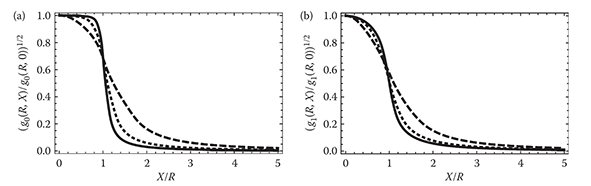
\includegraphics{Figures/LFP/LFP-how-local-outside-population-center-w100-r150}
\end{center}
\caption[]{Population LFP outside center of population. 
Left: Uncorrelated. Right: Correlated.
\gen{Figure and caption to be updated.
Maybe illustrate set up and "half-plane" argument.}
}
\label{LFP:fig:how-local-outside-population-center}
%\figpermOurs
\end{figure}
%%%%%%%%%%%%%%%%%%

When comparing the population LFPs for the uncorrelated and fully correlated cases in
Figure~\ref{LFP:fig:how-local-outside-population-center} we observe that 
relative to the amplitude recorded in the population center, the LFP amplitude at the 
population edge $\sigma(R,R)$ is larger for uncorrelated cases than the correlated cases.
This can be qualitatively understood by considering $\sigma(R,R)$ in the limit $R \rightarrow \infty$ where
being on the edge approaches the situation of being at the edge of an infinitely large half-plane. In this
situation, the recorded variance of the LFP at the center of the population will correspond to being in the middle
of an infinite plane, that is, the sum of the signal variance from two infinitely large half-planes. We thus have
$\sigma_\text{u}(R,0)^2=2\sigma_\text{u}(R,R)^2$, so that  $\sigma_\text{u}(R,R)/\sigma_\text{u}(R,0)=\sqrt{2} \simeq 0.71$. For the case with
$R=1$~millimetre in Figure~\ref{LFP:fig:how-local-outside-population-center}(a) we indeed observe 
$\sigma(R,R)/\sigma(R,0) \sim 0.7$ even though $R/r_*$ (which is the relevant measure) in this case
is only about 10 or so.

For the fully correlated case we find by the same argument that  $\sigma_\text{c}(R,0)=2\sigma_\text{c}(R,R)$ so that
$\sigma_\text{c}$ at the edge should be about half of  $\sigma_\text{c}$ in the population center when 
$R \rightarrow \infty$. And this is indeed close to what is observed for $R=1$~millimetre in 
Figure~\ref{LFP:fig:how-local-outside-population-center}(b). 

Close inspection of the large-$X$ tail of the population-LFP curves in Figure~\ref{LFP:fig:how-local-outside-population-center}
reveals a power law, that is, $\sigma(R,X) \sim 1/X^2$~\cite**[Figure~3.9]{Einevoll2013a}. For sufficiently large values of $X$, that is,
$X \gg R$, inspection of the integral expressions in Equations~\ref{LFP:equation:sigmaR2-X-uncorrelated-quantitative}  
and~\ref{LFP:equation:sigmaR2-X-correlated-quantitative} in fact reveals that in this limit the population LFP will exhibit the 
same large-X power-law behaviour as the single-neuron shape function $f(r)$, see \cite**{Einevoll2013a}.      


\section{\red{TVN/EH: Network LFPs}}
\begin{itemize}
\item Cortical LFPs from single corticothalamic neuron \cite**{Hagen2017}
\item Cortical networks with passive dendrites with hybrid trick \cite**{Hagen2016}
\item Cortical network with active dendrites \cite**{Reimann2013}
\end{itemize}

\section{\red{GTE: Insights from LFP studies}} 
